%\documentclass[a4paper,pra,twocolumn,amsmath,noamsfonts]{revtex4}
%\documentclass[a4paper,twocolumn,10pt]{iopart}

\documentclass[a4paper,10pt]{iopart}

\usepackage{setstack}
\usepackage{setspace}
\usepackage{wrapfig}
\usepackage{breqn}

\usepackage[amssymb]{SIunits} 
\usepackage{color}
\usepackage{ifthen}
\usepackage{xspace}
\usepackage{graphicx}

%\usepackage{pdfpages}
%\DeclareGraphicsExtensions{.eps}
%\DeclareGraphicsRule{.jpg}{eps}{.jpg.bb}{`jpeg2ps -h -r 600 #1}
%\usepackage{amsmath}%
%\usepackage{amsfonts}%
%\usepackage{amssymb}%

\newcommand{\be}{\begin{equation}}
%\newcommand{\bi}{\begin{itemize}}
\newcommand{\ee}{\end{equation}}
\newcommand{\ei}{\end{itemize}}
\newcommand{\ba}{\begin{eqnarray}}
\newcommand{\ea}{\end{eqnarray}}
\newcommand{\btd}{\bigtriangledown}
\newcommand{\pa}{\parallel}
\newcommand{\pe}{\perp}
\newcommand{\nn}{\nonumber}
\newcommand{\om}{\omega}
\newcommand{\g}{\gamma}
\newcommand{\gam}{\gamma}
\newcommand{\Om}{\Omega}
\newcommand{\vfi}{\varphi}
\newcommand{\ti}{\tilde}
\newcommand{\te}{\theta}
\newcommand{\de}{\delta}
\newcommand{\lbd}{\lambda}
\newcommand{\prt}{\partial}
\newcommand{\eps}{\epsilon}
\newcommand{\bfg}{\begin{figure}}
\newcommand{\ka}{\kappa}
\newcommand{\cpt}{\caption}
\newcommand{\efg}{\end{figure}}
\newcommand{\Ree}{\mathop{\mathrm{Re}}}
\newcommand{\Ima}{\mathop{\mathrm{Im}}}
\newcommand{\w}{\mathrm{w}}
\newcommand{\gys}{\textsc{Gysela}}%
\newcommand{\jor}{\textsc{Jorek}}%
\newcommand{\iter}{\textsc{Iter}}%
\newcommand{\xgc}{\textsc{XGC1}}%
%\newcommand{\PS}{Pfirsch--Schl\"uter}%
\newcommand{\GS}{Grad--Shafranov}%
\newcommand{\qlk}{\text{QuaLiKiz}}%
\newcommand{\gkw}{\textsc{gkw}}%
\newcommand{\gene}{\textsc{gene}}%
\newcommand{\gyro}{\textsc{gyro}}%
\newcommand{\gst}{\textsc{GS}2}%
% ------------------------
%   Coord 
% ------------------------
\newcommand{\x}{\mathbf{x}}%
\renewcommand{\b}{\mathbf{B}}%
\renewcommand{\v}{\mathbf{v}}%
\newcommand{\vpar}{v_\parallel}%    
\newcommand{\vparn}{{\vpar}/{\sqrt{2} v_T}}%
\newcommand{\upar}{u_\parallel}%           % uparallel
\newcommand{\uparn}{\frac{\upar}{v_{Ti}}}%
\newcommand{\uparns}{\frac{\upar}{v_{Ts}}}%
\newcommand{\gradu}{\nabla{u_\parallel}}%
\newcommand{\gradun}{\frac{R\gradu}{v_{Ti}}}%
\newcommand{\graduns}{\frac{R\gradu}{v_{Ts}}}%
% ------------------------
%   Maths
% ------------------------
\renewcommand{\d}{\mathrm{d}}%
\newcommand{\dt}{\partial_t}%
\newcommand{\dtheta}{\mathrm{d}\theta}%
\newcommand{\dx}{\mathrm{d}_x}%
\newcommand{\dr}{\mathrm{d}_r}%
\newcommand{\ddx}{\mathrm{d}_{xx}}%
\makeatletter
\DeclareRobustCommand\sfrac[1]{\@ifnextchar/{\@sfrac{#1}}%
                                            {\@sfrac{#1}/}}
\def\@sfrac#1/#2{\leavevmode\kern.1em\raise.5ex
         \hbox{$\m@th\mbox{\fontsize\sf@size\z@
                           \selectfont#1}$}\kern-.1em
         /\kern-.15em\lower.25ex
          \hbox{$\m@th\mbox{\fontsize\sf@size\z@
                            \selectfont#2}$}}%
 
                           
% ------------------------
%   Physics
% ------------------------
\newcommand{\ve}{\mathbf{v}_E}%              %v_E
\newcommand{\vg}{\mathbf{v}_d}%              %v_d
\newcommand{\ome}{\omega}%                   % omega
\newcommand{\omen}{\omega_{ne}^{\ast}}%      % Density diamagnetic frequency
\newcommand{\omepe}{\omega_{pe}^{\ast}}%     % Pressure diamagnetic
\newcommand{\omepi}{\omega_{pi}^{\ast}}%     % Pressure diamagnetic
\newcommand{\omeu}{\omega_{u}^{\ast}}%       % Velocity diamagnetic frequency
\newcommand{\omed}{\omega_d}%                % Vertical drift frequency
\newcommand{\kperp}{k_{\perp}}%              % kperp
\newcommand{\kpar}{k_{\parallel}}%           % kparallel
\newcommand{\kthe}{k_{\theta}}%              % ktheta
\newcommand{\n}{\mathbf{n}}%
\newcommand{\J}{\mathbf{J}}%
\newcommand{\OmeJ}{\n\cdot{\boldsymbol{\Omega}_\J}}% n.omega_J
\newcommand{\Omestar}{\n\cdot{\boldsymbol{\Omega^\ast}}}%     % n.omega*
\newcommand{\Omestars}{\n\cdot{\boldsymbol{\Omega}}_s^\mathbf{\ast}}% n.omega*_s
\newcommand{\exb}{\mathbf{E}\times\mathbf{B}}%
\newcommand{\zeff}{Z_{\textsl{eff}}}%
\newcommand{\gameff}{\gamma_{\textsl{eff}}}%
\newcommand{\omE}{\omega_{\exb}}%            %omega_ExB 
% -------------------
% Abbreviations diverses
% -------------------
\newcommand{\deff}{d_{\textsl{eff}}}
\newcommand{\ceff}{c_{\textsl{eff}}}
\newcommand{\reff}{\rho_{\textsl{eff}}}
\newcommand{\I}{\mathcal{I}}
\newcommand{\ds}{\displaystyle}
\newcommand{\ie}{\emph{i.e.}}
% ----------------------

\newcommand{\unitp}[3]{\unit{\nombre{#1}\times\power{10}{#2}}{#3}}

%% On affiche les figures ou pas ?
\newcommand{\figureouinon}{oui}

%% Commande synthetique & conditionnelle pour les figures
\newcommand{\myfigure}[4]{
  \ifthenelse{\equal{\figureouinon}{oui}}{ 
  \begin{figure}
    \includegraphics[#1]{#2}
    \caption{ \label{#3} #4}
  \end{figure}
  }{} %fin de ihthenelse
}

%%%% tableau math en mode displaystyle %%%%
\newenvironment{disarray}%
{\everymath{\displaystyle\everymath{}}\array}%
{\endarray}


%%%%%%%%%%%%%%%%%%%%%%%%%%%%%%%%%%%%%%%%%%%%%%%%%%%%%%%%%%%%%%%%%%%%%%%%%%%%%%%%%%%%%%%%%%%%%%%% 
%%%%%%%%%%%%%%%%%%%%%%%%%%%%%%%%%%%%%%%%%%%%%%%%%%%%%%%%%%%%%%%%%%%%%%%%%%%%%%%%%%%%%%%%%%%%%%%% 

\begin{document}

\section{Abstract}
Particle transport is fundamental in the optimization of a fusion device. The attention has rarely been on multiple isotope transport. Previous experiments, and in particular recent ones at JET, hinted towards larger diffusion coefficients for ion than for electrons. Theoretical work consistently predicted this behaviour for ITG dominated plasmas. The JET experiments were reproduced in this work using the framework of integrated modelling, with QuaLiKiz as the anomalous transport model. We were able to reproduce the experimental profiles and to retrieve the observed core isotope concentration. The phenomena appears to be robust against the choices that were made on physics and boundary conditions.


\section{Introduction}

Understanding and predicting particle transport is essential to interpret and optimize experiments. Most of the attention on this topic has historically been on the electron particle transport, and in particular on H-mode scenarios. [] The particle flux is usually formalized as 

$$ \Gamma = D \frac{dn}{dr} + nV + 1/D int sorgente $$

with $ D $ the diffusion coefficient and $ V $ the pinch. The diffusion is experimentally found to be much larger than the neoclassical predictions, so the community agrees that the origin of the particle transport is turbulent [?]. A turbulent pinch was also proved [], being more or less important for the density peaking depending on the conditions.

Less effort was put on the ion channel, since thanks to ambipolarity the total ion and electron transport have to be equal. This is not as trivial when multiple ions are considered, since they can mix without affecting the electron density. Previous works, in fact, already suggested a more complicated story. Fast isotope mixing was observed in TFTR [], experiments at JET showed fast tritium profile [], large He transport was observed by both modelling and experiments [].

Recent experiments at JET were performed with two main ion species, Hydrogen and Deuterium []. The core isotope sources were varied by scanning the relative contribution of peripheral gas injection (edge source) and neutral beam injection (core source). The explicit goal was to understand the dependency of the core particle source on the different isotopes peaking. The edge composition was measured comparing the relative amplitude of Balmer $ H_{\alpha} $ and $D_{\alpha} $ spectral lines, while the Deuterium density was derived indirectly from the neutron rate.

It was found that for both isotopes the density in the core was larger than at the edge. This is commonly referred as density peaking and was observed despite the core source being only Deuterium or only Hydrogen. A closer look on equation 1 shows how a large diffusion coefficient could explain the apparent insensitivity of the isotope profiles to the source. This would at the same time, for a peaked density, imply a large pinch.

At the level of collisionality of those experiments the theory predicts a large contribute from the NBI to the density peaking. This also means that, at least for electrons, those coefficients need to be small. In this view, diffusion and pinch can be larger for ions than for electrons.

Following the experimental work, it was shown that it is possible for this coefficients to be large, while still maintaining ambipolarity, for example in the situation of a strong ion diffusion balanced by a strong pinch []. In a single isotope plasma it is impossible to notice this effect, but there are implications in the presence of multiple ions.

The theoretical reason for the difference in the coefficients was then investigated with nonlinear and quasilinear simulations, down to a simple analytical model where it becomes evident that it is due to a resonant process []. The resonance changes depending on the leading turbulence, having opposite effects for Ion Temperature Gradient (ITG) and Trapped Electron Mode (TEM). For the latter the electron coefficients are in fact larger than the ion ones. The experiments at JET were actually found to be ITG dominated, so in line with the theoretical predictions.

This means that it is important to always specify whether the focus is on the ion or the electron particle transport channel. There will be two different timescales and there will be an important difference between ITG and TEM dominated regimes. This has consequences for isotope control and for helium ash removal.

In this work, we reproduce this experimental results in the framework of integrated modelling, using the JINTRAC suite [] with QuaLiKiz [] as the turbulent transport model. We show that we can reproduce the experimental temperature and density profiles, which give us confidence that the correct ITG regime is being captured. We then show that we can obtain quantitative agreement with the experimental Deuterium profiles and that the phenomena is robust and quite insensitive to the boundary conditions and physical hypothesis in the model.

\section{Tools and methods}

Multi-channel integrated modelling is a very powerful tool in reproducing the experiments. It allows to capture the complicated and nonlinear interactions between the various codes, as well as efficient comparison on multiple profiles. In addition to the reproduction of experimental results, the modelling was performed with two more goals in mind. One was to assess the robustness of the main results against the various choices that had to be made on the physics, the codes and on the boundary conditions. The second was to move towards fully predictive and self-consistent simulations, in preparation of extrapolation in different conditions.

This fast isotope mixing is in fact planned to be used in a full power scenario, where a pure tritium plasma will be fueled with pure Deuterium beams. Provided that the Deuterium does not accumulate in the core, the beam-thermal reactions should be maximized. Since most of the fusion power in mid-sized tokamaks comes from this channel, such scenario could be a viable way to reach the 16MW goal at JET. (Move later?)

The focus of this work is on the three discharges presented in table --. In particular, $\#91227$ and $\#91232$ were the object of a careful experimental comparison. While is normally impossible to measure Ds and Vs separately in steady state, it is shown that it becomes possible for multiple - isotope plasmas. The core Deuterium concentration and the transport coefficients retrieved by the analysis are reported in table --. 

The nonlinear simulations that followed the experimental work were performed with GKW []. The first principle based - quasilinear turbulent transport model QuaLiKiz [] was then used to reproduce the results from nonlinear simulations and good agreement was observed in the $D_{i}/D_{e} $ ratio. The speed of QuaLiKiz allows it to be used in integrated modelling and specifically in JETTO []. The goal was then to quantitatively reproduce the experiments in a flux driven simulation. 

The initial profiles were obtained using a Gaussian Regression Process tool available at JET []. GPR provides both fit and derivative uncertainties and it is expecially suited for comparison with the experiments. The electron temperature and density were obtained from the HRTS, while ion temperature and rotation were obtained from edge and core charge exchange. The experimental data were averaged for $ \sim 400 ms $ during flat - top.  The experiments are supposed to be in steady state, since all the kinetic profiles were not changing significantly for several confinement times. A steady state was also reached in the simulation by letting the profiles relax for 2s, corresponding to $ \sim 10 $ particle confinement times. Special care was taken for the equilibrium evolution, since the timescale for the current diffusion can be large.

In JINTRAC there is the possibility to couple JETTO to EDGE2D and do a self-consistent core-edge simulation, but due to the computational time required it was chosen not to model the edge. The pedestal was also taken from the experiment, since the use of EPED would have been an unecessary complication at this stage. The boundary conditions were therefore taken at $ \rho = 0.8 $ from the GPR fit. We self-consistently predicted the electron and ion temperature ($T_{e}, T_{i}$), the electron, Hydrogen, Deuterium and Berillium density ($n_{e}, n_{H}, n_{D}, n_{Be}$) and the rotation ($\Omega $). The neoclassical and turbulent transport were calculated with NCLASS [] and QuaLiKiz. The levels of radiation were always low ($P_{rad} \simeq 1MW $), so it was decided not to use NEO and not to simulate the Tungsten transport.

The neutral source at the edge was calculated with FRANTIC [], the NBI heating profile with PENCIL [], the impurities transport with SANCO [], the equilibrium and current transport with ESCO [] and NCLASS. Sawteeth are not modeled, despite the availability of a Sawteeth model in JETTO. There are still some uncertainties in the transport mechanisms inside $\rho < 0.2 $ [?] and the Sawteeth slow down the simulations, so we simply decided to consider the simulation unrealiable for $\rho > 0.2 $. Extra transport coefficients were added there to match the experiment.

It is worth noticing that the simulations are, a part from the impurity content and the top of the pedestal boundary conditions, indipendent from the experiment, in principle not different from a predict - first approach. All the simulations use the same settings, with no simulation-dependent fitting parameters.

\section{Modelling assumptions}

There are multiple aspects in the setting up of the simulations that require special care. The decisions made in this process are presented below.

\subsection{Boundary conditions}

As will be explained in more details later, the values of density and temperature at the top of the pedestal have an influence on the simulated profiles. This means that special attention is necessary for the experimental values close to the top of the pedestal. For the discharges presented in this work, for example, a misalignment [Lorenzo Frassinetti] of one of the HRTS systems prevented us to use some of the data. The Thompson Scattering data in $ 0.75 < \rho < 0.85 $ were not included in the GPR fits.

Edge charge exchange (CX) was only available in $\#91754$, while just core CX was available in $\#91232$ and $\#91227$.The ratio between $T_{i}$ and $T_{e}$ was found to have a huge impact on the density peaking[Oliver]. A correct extimation of $T_{i}$ at $ \rho = 0.8 $ is then crucial to reproduce the density peaking. Core CX is not always precise at the edge and for $\#91754$ it overpredicts $T_{i}$ with respect to the edge CX [is there an article for the difference between impurity CX and main ion CX? Is this what I am seeing here?]. In such relatively low power - high collisionality discharges $T_{i}$ is usually supposed to be very similar to $T_{e}$, and that is actually the value measured by edge CX. For this reason, core CX was supposed to be overestimated at the edge also for $\#91232$ and $\#91227$. $T_{i} = T_{e}$ at $ \rho = 0.8 $ was set for all the discharges.

\subsection{Sources}

PENCIL [] was used for the electron and ion heat source, as well as the core particle source. The total power was set to be equal to the experimental one.

The edge neutral source was calculated by FRANTIC []. An efficiency of --- percent was used. A standard method to measure the efficiency is not available, but some assumptions can be made. It has to be below the maximum puffing, and it is usually quite low, around 10 percent of that value [If I remember correctly it was Francis saying this, after some modeling done by Luca. Should probably send a mail for references here]. It was calculated in [] as …, obtaining --- percent%.

\subsection{Equilibrium}

The kinetic profiles are heavily depend on the magnetic shear, so an accurate equilibrium reconstruction is mandatory. Unfortunately only the standard EFIT [] was available, with the Q profile larger than 1 over the whole profile even though sawteeth were present in the experiments. Again trying to be as indipendent from the experiment as possible, ESCO was used for the equilibrium. The experimental internal inductance was observed to be rather constant for a timescale larger than the current evolution timescale, so the current profile was supposed to be relaxed. 
The initial profile was obtained from EFIT and then relaxed in a simulation with fixed temperature and density profiles but predictive current. Since in the experiment Sawteeth were present, the Sawteeth model in JETTO was used in this preliminary simulations. The relaxed profiles with and without Sawteeth were different enough to justify this choice.
The parameters in the sawteeth model were found not to be very important for the final current profile, so the default ones were used. This relaxed q profile was the one chosen for the Basecase. The difference between the internal inductance in the experiment and the one abtained with this method is around 5 percent. The impact of the equilibrium on the results will be discussed in chapter 3.

\subsection{Impurities}

Low concentration of multiple impurities were found in all the discharges, but only Beryllium was used. Beryllium should in fact be the largest contribution to the dilution. $ Z_{eff} $ and dilution have the largest impact on the kinetic profiles, so by matching  $ Z_{eff} $ with Beryllium we can account for impurities.
Tungsten contribution to dilution and  $ Z_{eff} $ is almost negligible, but is basically the only source of radiation. Since radiation from the core is less than 1MW in all cases, it has very little effect on the profiles. Tungsten modelling requires NEO and greatly slows down the simulations, so it was decided not to include it. A flat radiation profile was used as a first approximation.

\subsection{QuaLiKiz settings}

Electron Temperature Gradient (ETG) driven turbulence was found to carry a large part of the electron heat flux in all cases, so the electron scale was always included.
QuaLiKiz is an electrostatic code. Since the expected level of EM stabilization is strongly correlated with the fast ion content in discharges with strong NBI heating [], an ad-hoc correction was applied to try to reproduce this effect. The normalised ion temperature gradient passed to QuaLiKiz, $ R/L_{T_{i}} $ , was multiplied by the ratio of the local thermal energy density over the local total energy density, $ W_{th}/W_{tot}$. This basically leads to an increase of the ion temperature and, even if it is not first principle, it usually provides better results in JET discharges.

The impact of rotation on the turbulence was included for $ \rho > 0.5 $. This because ??? . The possibility of introducing the fast ions as an extra Maxwellian specie is being considered, but since it has not yet reached agreement with more complete codes it was decided not to include it.
(Fast ion story here). The ETG scale was included in all cases.

The result of the simulations for the three cases are shown in figure 1, 2, 3. The core deuterium concentration from the experiments is -- -- -- [Maslov]. Discrepancies between the model and the experiment will be discussed in more details in chapter 3. It is worth to notice that in all cases, as anticipated, both isotope profiles are peaked even if the core source is only on Deuterium or Hydrogen. The ratio of the coefficients for the last timestep in $\#91754$ is shown in figure 4. It’s similar in the other cases and it’s not reported for brevity. Between the experimental errors the basecase matches the deuterium content in all the considered discharges.

\begin{figure}
	\centering
	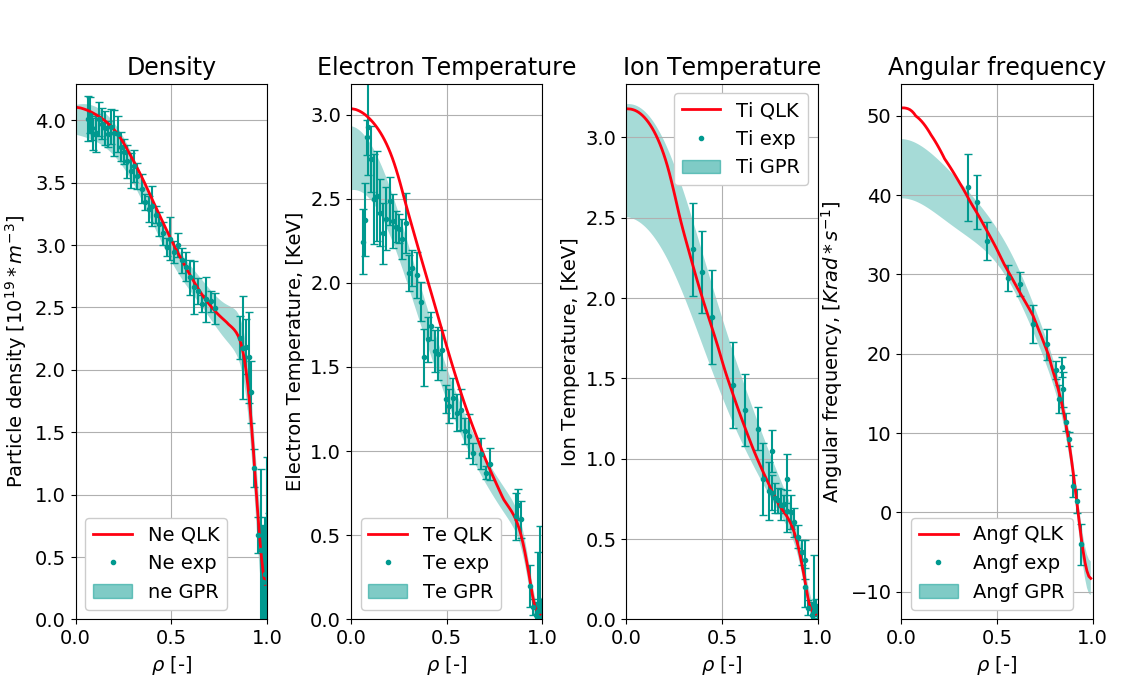
\includegraphics[width=0.9\linewidth]{Plots/91754}
	\caption{}
	\label{fig:91754}
\end{figure}

\begin{figure}
	\centering
	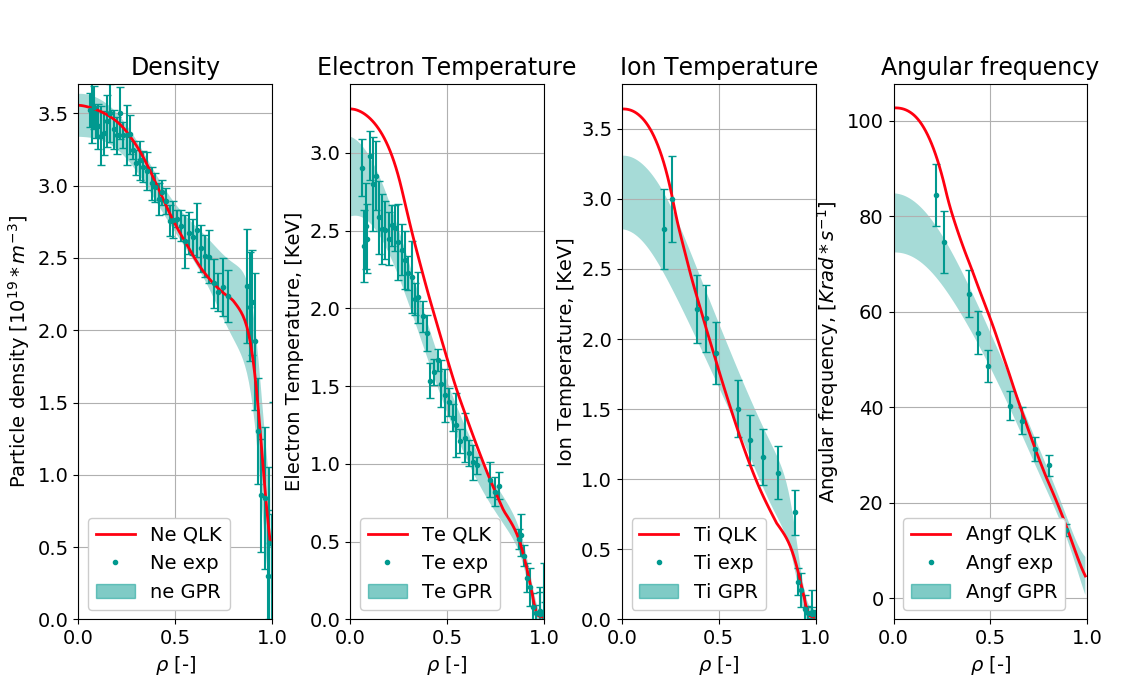
\includegraphics[width=0.9\linewidth]{Plots/91232}
	\caption{}
	\label{fig:91232}
\end{figure}

\begin{figure}
	\centering
	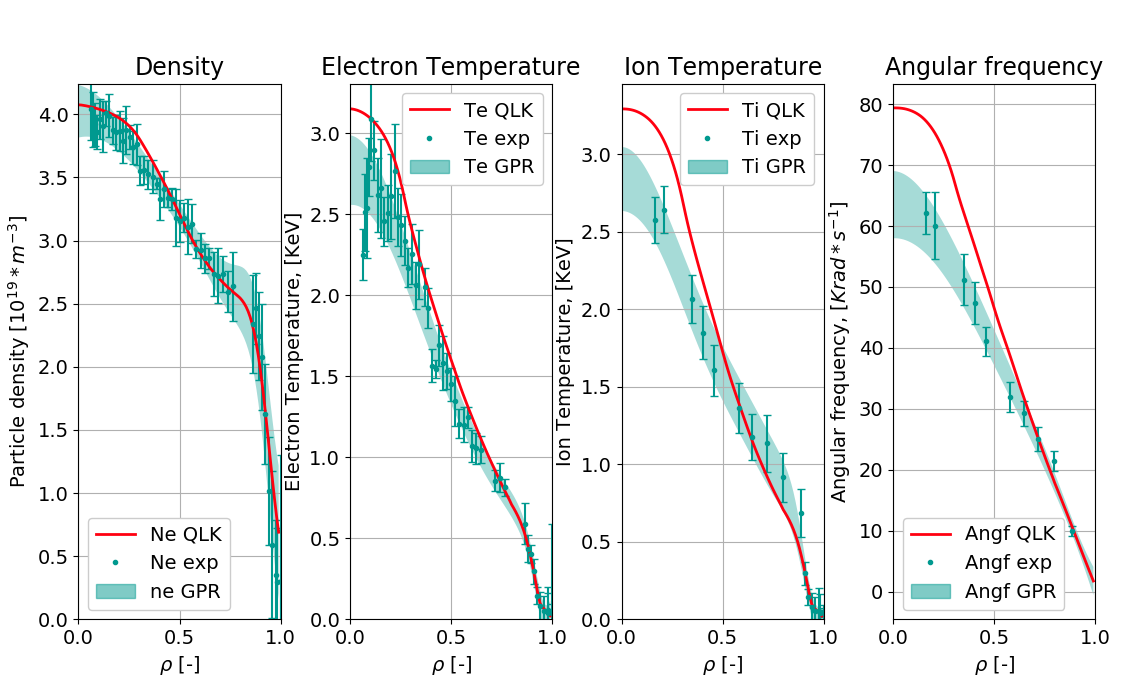
\includegraphics[width=0.9\linewidth]{Plots/91227}
	\caption{}
	\label{fig:91227}
\end{figure}


\section{Chapter three}

A sensitivity scan was performed to show that the phenomena under consideration is not dependent on any of the modelling assumptions. This also allows us to check the origin of eventual discrepancies between the model results and the experimental data. The impact of boundary conditions, codes used, physics assumptions and modelling choices is presented here.

As anticipated in Chapter 2, the largest sensitivity regarding the boundary conditions is on the $ T_{i}/T_{e} $ ratio. Larger $ T_{i}/T_{e} $ destabilizes ETG and stabilizes ITG, decreasing the particle outward diffusion. In this case where the NBI particle source is important, this translates in a more peaked density for higher $ T_{i}/T_{e} $. The temperatures, thanks to the stiffness of the heat transport, do not change significantly. 

When $ T_{i} $ and $ T_{e} $ are changed at the same time, on the other hand, there is very little change on the temperature and density gradients. Changing the density boundary condition also has little effect, rising the average density but without really impacting the gradients. The effect of the boundary conditions on the profiles is shown in figure --.

Changes in the total NBI power or in the ion - electron heating ratio, when not drammatic, proved not to be important in determining the final profiles. Regarding the edge neutrals source calculated with FRANTIC, even when raised to unrealistic values it could not change the $ \frac{n_{D}}{n_{H} + n_{D}} $ more than 1 percent. An imprecision in the sources calculation would not therefore impact our results.

$ Z_{eff} $ was very low in all the cases considered, below 1.2, but it is still important to consider impurities. Higher $ Z_{eff} $ is stabilizing for ITG and expecially for ETG (can I state it like this or I need plots and a few lines to explain it better? Or should I not mention it at all?), so even for these low concentration there is an impact on the electron temperature. Impurities are to be considered in the comparison with the experiment, but it is important to notice that nor dilution nor the effect on $ T_{e} $ were found to modify the $ \frac{n_{D}}{n_{H} + n_{D}} $ ratio.
The radiation can in principle modify the density peaking, but only when the levels of radiation are comparable with the electron heating, which was not the case in the experiments that were considered. Since most of the radiation is due to tungsten and since tungsten, due to its high charge, does not contribute strongly to $ Z_{eff} $ or to the dilution, a limited effect of the radiation means a limited effect of tungsten. Doubling the radiation had very little effect on the profiles (fig something?), thus justifying the choice not to model tungsten.

Including the ETG scale is essential to be able to correctly predict the electron temperature, that is grossly overestimated otherwise. This is shown in figure ??.

The ad hoc 'electromagnetic' stabilization, given the large fraction of fast ions pressure (how much here?), has a strong impact on the profiles. The ion temperature is increased, and given the relatively high collisionality the electron temperature increases as well. The $T_{i}/T_{e} $ ratio also changes, and as it was explained before this modifies the density peaking. There is in this case an effect on the $ \frac{n_{D}}{n_{H} + n_{D}} $ ratio, since it seems to correlate with the density peaking. The effect on the ratio is not large enough to contradict the main point, but suggests that this is an important parameter to consider in this analysis.

A correct equilibrium reconstruction is also necessary when trying to capture the experimental profiles. The q profile and the magnetic shear, through the $s/q $ ratio, have a strong impact on the ITG and ETG threshold. The sensitivity from the point of view of integrated modelling is shown in figure ??. In the q profile obtained with EFIT the value of q is clearly overestimated in the core, since sawteeth are measured in the discharge. Supposing similar boundary conditions, as is the case, this also means overestimated shear. In the simulation where the current is predicted, on the countrary, the shear monotonically increases as the simulation evolves. The two cases can be therefore taken as two extreme cases.

The pulse with the largest variation between edge and core D concentration is, unsurprisingly, 91232. In this case there is no Deuterium puffing and its concentration is at the lowest. The relative intensity of the source is the largest when compared to the Deuterium density, so a larger impact is expected.

The kinetic profiles can have rather strong (do not say this, use the actual numbers) dependencies on the assumptions, but the $ n_{D}/(n_{D}+n_{H}) $ ratio never changes more than a couple of percentages. The density peaking itself can change considerably, as it is shown in table []. Even when this happens, once the ratio is fixed at the edge it is very difficult to change it, at least in the model. Both deuterium and hydrogen are found to be peaked in all cases and the phenomena is robust against the assumptions.

\begin{figure}
	\centering
	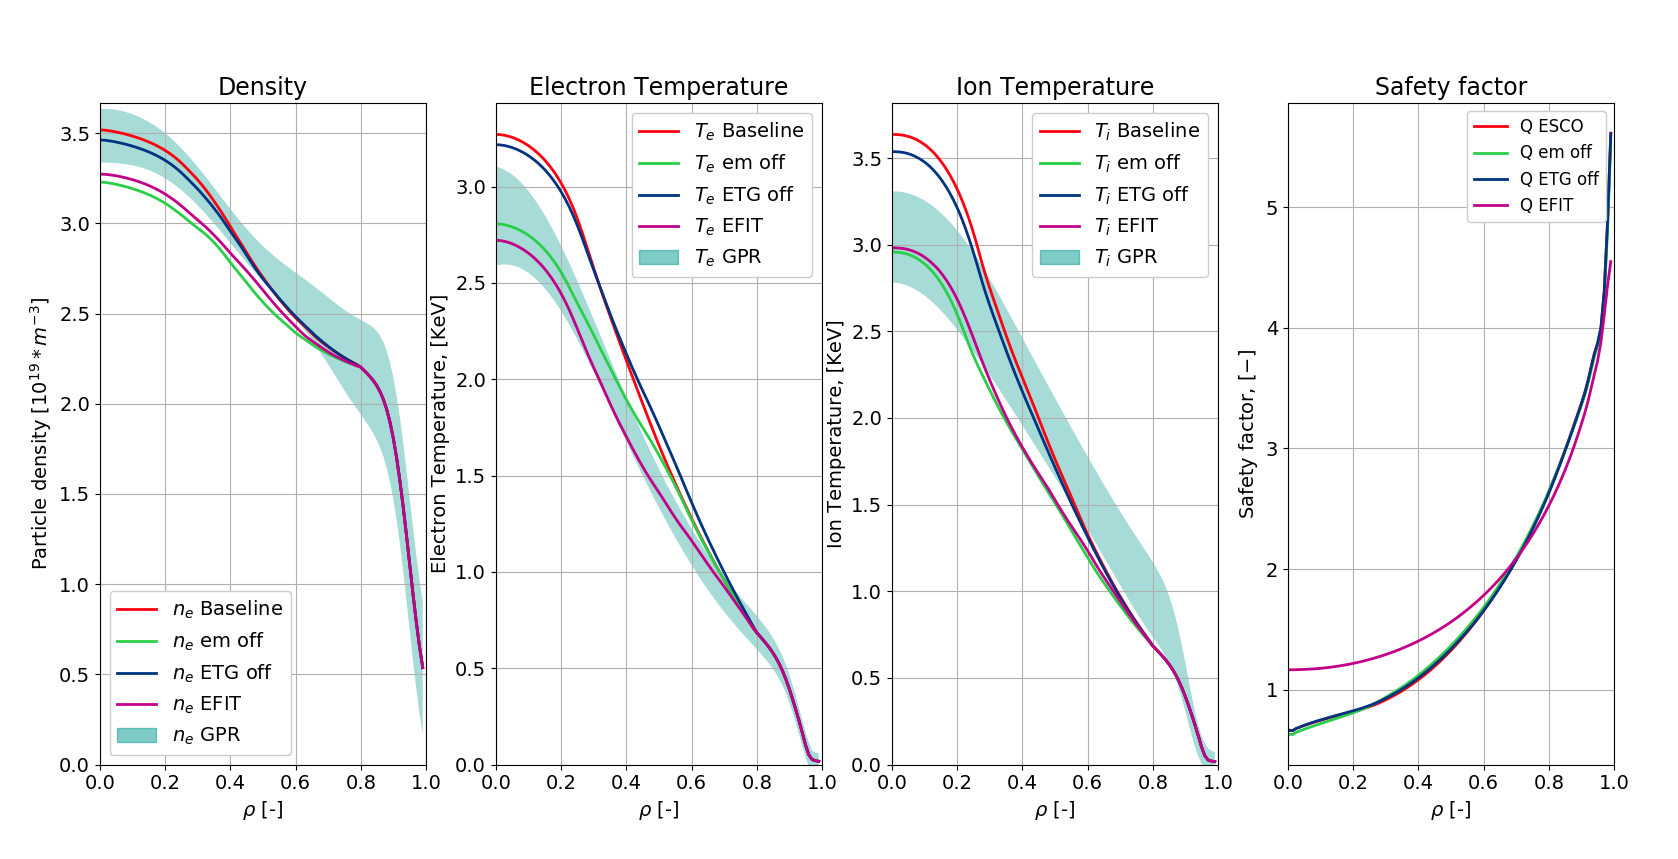
\includegraphics[width=0.9\linewidth]{Plots/91232_sensitivities}
	\caption{}
	\label{fig:91232sensitivities}
\end{figure}

\begin{figure}
	\centering
	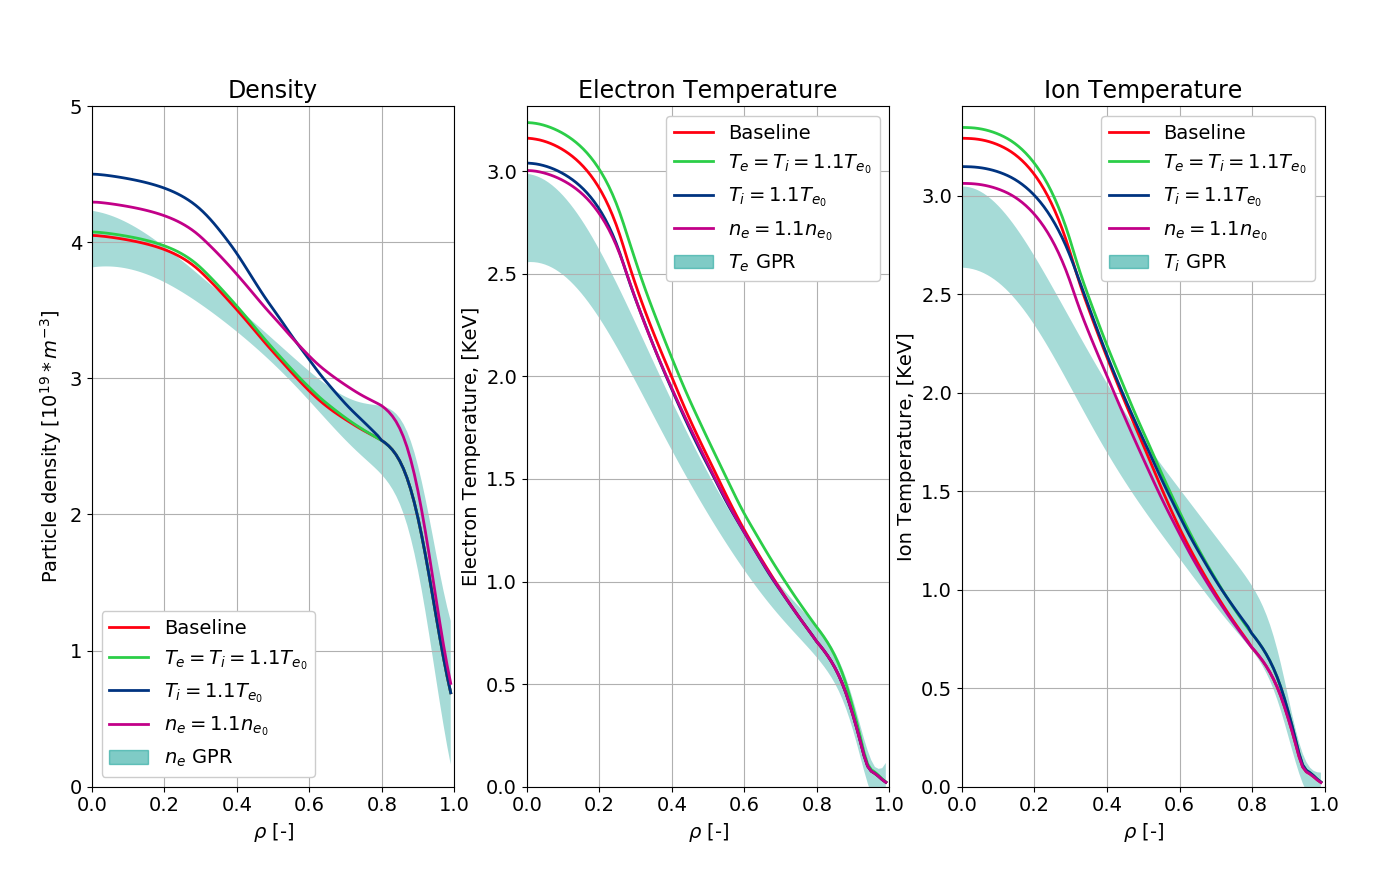
\includegraphics[width=0.9\linewidth]{Plots/91227_Ti_Te}
	\caption{}
	\label{fig:91227tite}
\end{figure}


\section{Conclusions}

We show how the fast isotope mixing implies peaked density profiles (following the electrons?) regardless of the core particle source. We also show that we are able to reproduce the experimental profiles inside the experimental errors for the boundary conditions and the equilibrium. Even though the profiles do depend on the modelling assumptions, the $ n_{D}/(n_{D}+n_{H}) $ ratio never changes consistently. This means that this effect is robust and can be predicted to appear in general for ITG dominated plasmas. 
This has implications for fueling, since maintaining the isotope ratio at the edge is enough to control it in the core. It is also has positive implications for Helium ash removal, since even if the peaking of the Helium profile could be unfavorable, the source would not affect it and make it worse. 





\singlespacing
\bibliographystyle{unsrt}
%\bibliography{references_from_endnotes_0915}

\end{document}
